%    This is appendices with specific sections.

\appndxsec{Important Notes}{\label{app:importantnotes}}

You always need to use a blank line between paragraphs to indicate a new paragraph otherwise the compiler will merge the two paragraphs together as one. Refer to the \texttt{tex} file for demonstration.

Similarly, for equations you need to have a blank line before and after them, otherwise it will overlap with the previous paragraph.

The first paragraph of every chapter should be written under the chapter declaration without any extra line breaks; otherwise it will cause some spacing issues with the next section.

Contents below are for test only.

\begin{definition}[]
Let $U$ be the domain of discourse
\end{definition}

\begin{table}[htb] % [htb] to be after the paragraph
\caption{A table for the Appendix \ref{app:importantnotes} to test the appendix captions.}
\label{table:3}
\begin{tabular}{|c c c c|}
 \hline
 Col1 & Col2 & Col2 & Col3 \\ [0.5ex]
 \hline\hline
 1 & 6 & 87837 & 787 \\
 2 & 7 & 78 & 5415 \\
 3 & 545 & 778 & 7507 \\
 4 & 545 & 18744 & 7560 \\
 5 & 88 & 788 & 6344 \\ [1ex]
 \hline
\end{tabular}
\end{table}

\begin{equation}\label{eqa}
G_{\mu \nu }=8\pi GT_{\mu \nu }
\end{equation}

\appndxsec{Second Appendix with yet Another Really Long Title to Test Multi-line Titles}{\label{app:titlecheck}}

This appendix is solely for testing the table, figure, and equation numbering.

\begin{figure}[!b]
    \centering
    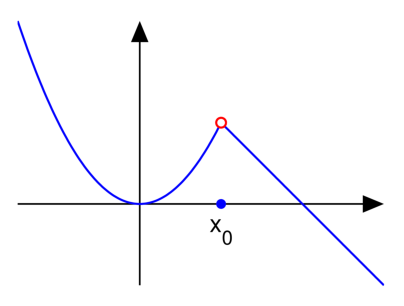
\includegraphics[scale=1.5]{figures/Discontinuity_removable}
        \caption{\centering Removable discontinuity, but it is scaled to 1.5 times the size of the original figure.}
    \label{fig:disc2}
\end{figure}

\begin{table}[b!] % [b!] to be at the bottom
\caption{Appendix \ref{app:titlecheck} table.}
\label{table:4}
\begin{tabular}{|c c c c|}
 \hline
 Col1 & Col2 & Col2 & Col3 \\ [0.5ex]
 \hline\hline
 1 & 6 & 87837 & 787 \\
 2 & 7 & 78 & 5415 \\
 3 & 545 & 778 & 7507 \\
 4 & 545 & 18744 & 7560 \\
 5 & 88 & 788 & 6344 \\ [1ex]
 \hline
\end{tabular}
\end{table}

\begin{equation}\label{eqb}
G_{\mu \nu }=8\pi GT_{\mu \nu }
\end{equation}

\begin{eqnarray}
  \sum \vert M^{\text{viol}}_g \vert ^2
   &=&  g^{2n-4}_S(Q^2)~N^{n-2} (N^2-1)
\nonumber
\\
   &&   \times \left( \sum_{i<j}\right) \sum_{\text{perm}}
            \frac{1}{S_{12}}  \frac{1}{S_{12}} \sum_\tau c^f_\tau
\,.
\label{eq:multilineeq2}
\end{eqnarray}

\begin{equation} \label{eu_eqn2}
e^{\pi i} + 1 = 0
\end{equation}

\begin{multline*}
p(x) = 3x^6 + 14x^5y + 590x^4y^2 + 19x^3y^3\\
- 12x^2y^4 - 12xy^5 + 2y^6 - a^3b^3
\end{multline*}

\begin{align*}
p(x) = 3x^6 + 14x^5y + 590x^4y^2 + 19x^3y^3\\
- 12x^2y^4 - 12xy^5 + 2y^6 - a^3b^3
\end{align*}

\begin{table}[htb]
\caption{Another appendix table.}
\label{table:5}
\begin{tabular}{|c c c c|}
 \hline
 Col1 & Col2 & Col2 & Col3 \\ [0.5ex]
 \hline\hline
 1 & 6 & 87837 & 787 \\
 2 & 7 & 78 & 5415 \\
 3 & 545 & 778 & 7507 \\
 4 & 545 & 18744 & 7560 \\
 5 & 88 & 788 & 6344 \\ [1ex]
 \hline
\end{tabular}
\end{table}
